%%%%%%%%%%%%%%%%%%%%%%%%%%%%%%%%%%%%%%%%%%%%%%%%%%%%%%%%%%%%%%%%%%%%%%%%%%%%%%%%
%                   PLANTILLA DE ARTÍCULO CIENTÍFICO - REVISTA +INGENIO
%                   Facultad de Ingeniería - UNaM
%%%%%%%%%%%%%%%%%%%%%%%%%%%%%%%%%%%%%%%%%%%%%%%%%%%%%%%%%%%%%%%%%%%%%%%%%%%%%%%%
% Este archivo .tex sirve como guía y plantilla de edición. 
% Se recomienda compilar con pdflatex + biber (para la bibliografía).
% Todos los estilos requeridos están pre-configurados en este preámbulo.
%%%%%%%%%%%%%%%%%%%%%%%%%%%%%%%%%%%%%%%%%%%%%%%%%%%%%%%%%%%%%%%%%%%%%%%%%%%%%%%%

% ==============================================================================
% 1. CLASE DE DOCUMENTO Y DIMENSIONES
% ==============================================================================
% \documentclass define el tipo de documento. 'article' es el estándar para artículos.
% - a4paper: Establece el tamaño de hoja estándar A4.
% - 12pt: Define el tamaño base de la tipografía.
\documentclass[a4paper, 12pt]{article}

% ==============================================================================
% 2. PAQUETES GRÁFICOS Y DE NAVEGACIÓN
% ==============================================================================
% \usepackage{graphicx} permite incluir imágenes en el documento.
% - Documentación del paquete: https://ctan.org/pkg/graphicx
\usepackage{graphicx} 

% \usepackage{hyperref} habilita los hipervínculos dinámicos y marcadores PDF.
\usepackage{hyperref} 
\hypersetup{
  colorlinks=true,       % Colorea el texto de los enlaces en lugar de poner recuadros.
  linkcolor=black,       % Color para referencias internas (secciones, figuras, tablas).
  filecolor=magenta,     % Color para enlaces a archivos locales.
  urlcolor=blue,         % Color para hipervínculos externos (URLs).
}

% ==============================================================================
% 3. IDIOMA Y CARACTERES
% ==============================================================================
% babel con opción 'spanish' configura la traducción automática de términos (e.g. "Abstract" -> "Resumen")
% y las reglas de división silábica al español.
\usepackage[spanish]{babel}
\usepackage{csquotes}    % Recomendado para comillas automáticas dependientes del idioma.

% ==============================================================================
% 4. PIES DE IMAGEN Y TABLAS (CAPTIONS)
% ==============================================================================
% \usepackage{caption} permite personalizar las leyendas de figuras y tablas.
\usepackage{caption}
\captionsetup{
  justification=centering, % Centra los pies si ocupan más de una línea.
  labelsep=period,        % Separa el número de la leyenda con un punto (.) en lugar de dos puntos (:).
  font={bf,footnotesize}  % Leyenda en negrita (bf) y tamaño reducido (10pt).
}
\addto\captionsspanish{
  \renewcommand{\figurename}{Fig.}   % Abreviatura obligatoria para figuras en la revista.
  \renewcommand{\tablename}{Tabla}   % Etiqueta obligatoria para tablas.
}

% ==============================================================================
% 5. GEOMETRÍA Y MÁRGENES DE PÁGINA
% ==============================================================================
\usepackage[top=25mm,
bottom=15mm, 
left=25mm, 
right=15mm,
includefoot]{geometry}   % 'includefoot' asegura que el pie de página quede dentro de los márgenes útiles.

\setlength{\parindent}{5mm} % Establece la sangría al inicio de cada párrafo (5 mm).

% ==============================================================================
% 6. TIPOGRAFÍA Y FUENTES
% ==============================================================================
\usepackage{setspace}
\setstretch{1.15}        % Establece el interlineado del texto a 1.15.

% newtxtext y newtxmath cargan la tipografía Times New Roman para texto y matemáticas.
\usepackage{newtxtext}
\usepackage{newtxmath}

% ==============================================================================
% 7. UNIDADES Y MATEMÁTICAS AVANZADAS
% ==============================================================================
% siunitx proporciona una maquetación profesional y consistente de unidades físicas.
% - Documentación del paquete: https://ctan.org/pkg/siunitx
\usepackage{siunitx} 
\sisetup{locale=DE, inter-unit-product=\cdot} % Configuración regional (coma decimal) y producto de unidades con punto.

% \usepackage{nomencl} permite generar la lista de símbolos (nomenclatura).
% - Documentación del paquete: https://ctan.org/pkg/nomencl
\usepackage{nomencl}     
\usepackage{multicol}    % Permite trabajar a varias columnas.
\makenomenclature
\renewcommand{\nomname}{Símbolos}
\renewcommand{\nompreamble}{\vspace{-0.8em}\begin{multicols}{2}}
  \renewcommand{\nompostamble}{\end{multicols}}

% Pie de página y notas al pie
\usepackage{fancyhdr}
\pagestyle{fancy}
\fancyhf{}
% - Configuración del encabezado de página dinámico (visible a partir de la página 2):
%   Reemplace "Siglas del Nombre y Apellido completo del Primer Autor et al."
%   con las iniciales de los nombres y el apellido completo del primer autor (ej: "J. P. Pérez et al.").
\fancyhead[L]{\footnotesize \ifnum\value{page}>1 Siglas del Nombre y Apellido completo del Primer Autor et al. \fi}
\fancyfoot[C]{\footnotesize \thepage}
\renewcommand{\headrulewidth}{0pt}
% \renewcommand{\footrulewidth}{0.4pt}
\usepackage[bottom]{footmisc}

% \usepackage{enumitem} permite modificar los estilos y espaciados de las listas (itemize/enumerate/description).
% - Documentación del paquete: https://ctan.org/pkg/enumitem
\usepackage{enumitem} 
\setenumerate{label=\arabic*), wide=0pt, listparindent=1.25em, parsep=0pt}
\setlist[description]{font=\bfseries\itshape,leftmargin=0em,labelindent=2em}

% \usepackage{tabularray} proporciona tablas más limpias y potentes que tabular/array de forma automática.
% - Documentación del paquete: https://ctan.org/pkg/tabularray
\usepackage{tabularray} 
\UseTblrLibrary{varwidth}

% Formato secciones, subsecciones
\usepackage{titlesec}
\titleformat{\section}
{\normalfont\normalsize\bfseries}{\thesection.}{1em}{}
\titleformat{\subsection}
{\normalfont\normalsize\itshape}{\thesubsection.}{1em}{}
\titleformat{\subsubsection}
{\normalfont\normalsize\itshape}{\thesubsubsection.}{1em}{}

% Formato resumen
\renewenvironment{abstract}{%
  \vspace{1em}\footnotesize\noindent
  \textbf{\textit{\abstractname}\\\indent}{}}


% Referencias y Citación
% - Documentación del paquete biblatex: https://ctan.org/pkg/biblatex
\usepackage[backend=biber,style=ieee]{biblatex}
\renewcommand*{\bibfont}{\normalfont\footnotesize}
\addbibresource{references.bib}

% Banner + título
\title{\vspace{-4em}
\includegraphics[height=2cm]{images/logo_fio.png}\hspace{3cm}
\includegraphics[height=2cm]{images/logo_ingenio.png}\\\vspace{1em}
  \large\textbf{
    %%%%%%%%%%%%%%%%%%%%%%%%%%%%%%%%% T Í T U L O %%%%%%%%%%%%%%%%%%%%%%%%%%%%%%%%%%
    Título del Artículo
    %%%%%%%%%%%%%%%%%%%%%%%%%%%%%%%%%%%%%%%%%%%%%%%%%%%%%%%%%%%%%%%%%%%%%%%%%%%%%%%% 
  }}

% Autores
\author{\normalsize
  %%%%%%%%%%%%%%%%%%%%%%%%%%%%%%%%% A U T O R E S %%%%%%%%%%%%%%%%%%%%%%%%%%%%%%%%
  % - Reemplace los nombres de ejemplo por los autores reales de la investigación.
  % - Escriba el primer nombre y apellido(s) de forma completa, y las iniciales del segundo nombre (ej: "Juan P. Pérez").
  % - Utilice el comando \and para separar a cada autor. Esto organizará automáticamente la alineación.
  % - Coloque superíndices (ej: $^{1}$, $^{2,3}$) para vincular a cada autor con sus afiliaciones.
  % - Marque el autor para correspondencia con una nota al pie usando \footnote{Autor en correspondencia.} pegado a su superíndice.
  Nombre/s y Apellido/s$^{1}$\footnote{Autor en correspondencia.} \and \normalsize
  Nombre/s y Apellido/s$^{2}$ \and \normalsize
  Nombre/s y Apellido/s$^{3}$ \and \normalsize
  Nombre/s y Apellido/s$^{3,4}$ \and \normalsize
  Nombre/s y Apellido/s$^{3,5}$
  %%%%%%%%%%%%%%%%%%%%%%%%%%%%%%%%%%%%%%%%%%%%%%%%%%%%%%%%%%%%%%%%%%%%%%%%%%%%%%%% 
}

% Afiliaciones, en lugar de fecha
\date{\footnotesize{\textit{
      %%%%%%%%%%%%%%%%%%%%%%%%%%% A F I L I A C I O N E S %%%%%%%%%%%%%%%%%%%%%%%%%%%%
      % - Redacte las afiliaciones dentro de \date{\footnotesize{\textit{ ... }}}.
      % - Cada institución debe comenzar con su superíndice correspondiente (ej: $^{1}$, $^{2}$).
      % - Indique la afiliación en orden jerárquico: Universidad, Facultad, Departamento o Laboratorio, Ciudad, Provincia, País.
      % - Utilice la doble barra (\\) al final de cada institución para forzar el salto de línea.
      % - Al final, incluya la lista de correos electrónicos (e-mails) de todos los autores.
      $^{1}$Universidad Nacional de Misiones (UNaM). Facultad de Ingeniería. Dpto. de
      Ing. Industrial. Laboratorio de Gestión Tecnológica. Misiones, Argentina \\
      $^{2}$Universidad Nacional de Misiones–CONICET. Facultad de Ingeniería.
      Instituto de Materiales de Misiones (IMAM) Grupo de Investigación y Desarrollo
      en Electrónica (GIDE). Oberá, Misiones, Argentina \\ 
      $^{3}$Universidad Amazónica del Ecuador (UAE). Facultad de Ingeniería. Dpto. de
      Industrias. Ecuador \\
      e-mails: emailauthor1$^{1}$, emailauthor2$^{2}$, emailauthor3$^{3}$,
      emailauthor4$^{4}$, emailauthor5$^{5}$
      %%%%%%%%%%%%%%%%%%%%%%%%%%%%%%%%%%%%%%%%%%%%%%%%%%%%%%%%%%%%%%%%%%%%%%%%%%%%%%%% 
    }}}

% ==============================================================================
%                      INICIO DEL DOCUMENTO PRINCIPAL
% ==============================================================================
% Todo el texto visible debe ir entre \begin{document} y \end{document}.
\begin{document}

% \maketitle genera de manera automática el título, autores y afiliaciones definidos arriba.
\maketitle
\thispagestyle{fancy}    % Aplica el estilo de cabecera/pie de página a la primera página.

\vspace{-1em}\hrule
\begin{abstract}\vspace{-2em}\singlespacing{
    %%%%%%%%%%%%%%%%%%%%%%%%%%%%%%%% R E S U M E N %%%%%%%%%%%%%%%%%%%%%%%%%%%%%%%%%
    Estas instrucciones constituyen una guía para la preparación de artículos
    científicos de la revista +Ingenio. Los autores deben utilizarla para escribir
    tanto la versión inicial y como la final del artículo. Se recomienda aplicar
    este documento como una “plantilla” para preparar su manuscrito. La información
    adicional para la preparación del artículo, el envío y posterior publicación,
    pueden obtenerse en este documento, con el editor principal vía e-mail o en el
    sitio web: http://revistas.fio.unam.edu.ar/index.php/ingenio. El Resumen debe
    presentar: el objetivo del trabajo, principales materiales, métodos, resultados
    y conclusiones; además no debe tener más de 200 palabras, ninguna abreviatura,
    referencia, figura ni tabla.
    %%%%%%%%%%%%%%%%%%%%%%%%%%%%%%%%%%%%%%%%%%%%%%%%%%%%%%%%%%%%%%%%%%%%%%%%%%%%%%% 
  }

  \vspace{0.5em}\noindent\textit{\textbf{Palabras Clave} ---
    %%%%%%%%%%%%%%%%%%%%%%%%% P A L A B R A S   C L A V E %%%%%%%%%%%%%%%%%%%%%%%%%%
    Hasta 10 palabras en orden alfabético, primera letra en mayúscula y separadas
    por coma.
    %%%%%%%%%%%%%%%%%%%%%%%%%%%%%%%%%%%%%%%%%%%%%%%%%%%%%%%%%%%%%%%%%%%%%%%%%%%%%%%% 
  }\end{abstract}

\vspace{1em}\hrule
\renewcommand{\abstractname}{Abstract}
\begin{abstract}\vspace{-2em}\singlespacing{
    %%%%%%%%%%%%%%%%%%%%%%%%%%%%%%% A B S T R A C T %%%%%%%%%%%%%%%%%%%%%%%%%%%%%%%
    These instructions are presented to assist authors in preparing the manuscript
    for the +INGENIO journal. The authors should use these guidelines for preparing
    both the initial and final versions of their paper. In addition, the authors can
    use this document as a model to prepare your manuscript. Additional information
    about procedures and guidelines for publication can be obtained directly by
    e-mail with the editor in chief, or through the web site
    \url{http://revistas.fio.unam.edu.ar/index.php/ingenio}.
    %%%%%%%%%%%%%%%%%%%%%%%%%%%%%%%%%%%%%%%%%%%%%%%%%%%%%%%%%%%%%%%%%%%%%%%%%%%%%%% 
  }

  \vspace{0.5em}\noindent\textit{\textbf{Keywords} ---
    %%%%%%%%%%%%%%%%%%%%%%%%%%%%%%% K E Y W O R D S %%%%%%%%%%%%%%%%%%%%%%%%%%%%%%%%
    Up to 10 keywords in alphabetical order, first letter capitalized and separated
    by commas.
    %%%%%%%%%%%%%%%%%%%%%%%%%%%%%%%%%%%%%%%%%%%%%%%%%%%%%%%%%%%%%%%%%%%%%%%%%%%%%%%% 
  }\end{abstract}
\vspace{1em}\hrule

%%%%%%%%%%%%%%%%%%%%%%%%%%%%%%%% S Í M B O L O S %%%%%%%%%%%%%%%%%%%%%%%%%%%%%%%
% Para agregar nuevos símbolos a la tabla, use la sintaxis: \nomenclature{<símbolo>}{<descripción>}
% Ejemplo: \nomenclature{$F$}{Fuerza (\si{\newton})}
\nomenclature{$S$}{Potencia aparente (TNR10)}
\nomenclature{$V_o$}{Tensión controlada de salida (unidades)}
\nomenclature{$V_i$}{Volumen inicial (\si{\litre})}
\nomenclature{$V_f$}{Volumen final (\si{\litre})}
\nomenclature{$P_p$}{Presión parcial (\si{atm})}
\nomenclature{$T_a$}{Temperatura absoluta (\si{\kelvin})}
\vspace{-0.8em}
\printnomenclature
%%%%%%%%%%%%%%%%%%%%%%%%%%%%%%%%%%%%%%%%%%%%%%%%%%%%%%%%%%%%%%%%%%%%%%%%%%%%%%%% 

\section{Formato del artículo}

La revista +INGENIO (Revista de Ciencia, Tecnología e Innovación de la Facultad
de Ingeniería, Universidad Nacional de Misiones), es un medio a través del cual
los investigadores pueden publicar sus trabajos científicos siguiendo el formato
aquí presentado. Los artículos científicos abarcan temas de interés, en el campo
de las ciencias técnicas en general y en particular de las ingenierías: Civil,
Electromecánica, Electrónica, Industrial, en Computación y Mecatrónica, entre
otras.

Se aceptarán trabajos en español, portugués e inglés, utilizando esta plantilla de \LaTeX{} o en el formato editable de \textbf{Word (Microsoft Office)}.

Los autores deben presentar su manuscrito electrónicamente y seguir el proceso
de revisión a través del sitio web de +INGENIO,
\url{https://revistas.fio.unam.edu.ar/index.php/masingenio/index}. Desde esta
página, se puede obtener acceso a toda la información necesaria para la
presentación del manuscrito.

\subsection{Presentación}

Los manuscritos presentados para su publicación en la Revista +Ingenio deberán
tener, preferentemente, entre 9 y 15 páginas a columna simple. Los autores deben
utilizar unidades del Sistema Internacional (SI o MKS). La revista no realizará
ningún formateo final del artículo. Su documento debe estar “listo para
publicarse” una vez aceptado.

\subsection{Ventajas de la Maquetación en \LaTeX{}}

La preparación de manuscritos en \LaTeX{} presenta múltiples ventajas frente a los procesadores de texto tradicionales (como \textbf{Word}), especialmente en el ámbito de las publicaciones científicas:
\begin{description}
  \item[Generación de hipervínculos:] El paquete \texttt{hyperref} convierte automáticamente todas las citas bibliográficas, referencias a ecuaciones, figuras, tablas y direcciones URL en hipervínculos interactivos clickeables dentro del documento PDF resultante.
  \item[Gestión de referencias:] La bibliografía se ordena y formatea automáticamente según el estándar IEEE a partir de la base de datos de referencias (\texttt{references.bib}), eliminando la necesidad de numerar y ordenar la lista de forma manual.
  \item[Consistencia tipográfica:] El autor se enfoca exclusivamente en la redacción del contenido, mientras que la plantilla gestiona de manera uniforme los márgenes, espaciados, fuentes y paginación a nivel global.
  \item[Calidad matemática:] El motor de composición de ecuaciones de \LaTeX{} es el estándar de la industria científica debido a su precisión gráfica en la renderización de símbolos y estructuras matemáticas complejas.
  \item[Control de versiones:] Al basarse en archivos de texto plano (\texttt{.tex}), los documentos en \LaTeX{} permiten el empleo eficiente de sistemas de control de versiones (como \textbf{Git}). Esto facilita el seguimiento detallado de cambios, la colaboración simultánea entre autores.
\end{description}


\subsection{Estructura del Proyecto y Archivos Clave}

Para la correcta edición de este manuscrito, se debe comprender la estructura del proyecto y la función de cada uno de sus archivos clave:
\begin{description}
  \item[main.tex:] Es el archivo fuente principal en formato \LaTeX{}. Contiene el preámbulo (donde se cargan los paquetes y configuraciones de formato de la revista) y el cuerpo del manuscrito estructurado en secciones. Toda la redacción y maquetación del artículo se realiza dentro de este archivo.
  \item[main.pdf:] Es el documento compilado final en formato PDF. Actúa como la guía de estilo visual y el manual de usuario de la plantilla. Este es el formato oficial requerido para la presentación definitiva del manuscrito a la revista.
  \item[references.bib:] Es el archivo de base de datos bibliográfica en formato BibTeX. Aquí se deben registrar todos los recursos y referencias utilizando la estructura normalizada de campos (como autor, título, año, revista, etc.), las cuales serán invocadas en el texto mediante \texttt{\textbackslash cite\{...\}}.
  \item[images/:] Directorio destinado a almacenar las imágenes y figuras utilizadas en el artículo (en formatos PDF, EPS, PNG o JPG). Se aconseja agrupar todos los recursos gráficos aquí para mantener organizado el espacio de trabajo.
  \item[Archivos temporales y de compilación:] Durante el proceso de compilación se generan diversos archivos auxiliares y de registro (como \texttt{.aux}, \texttt{.log}, \texttt{.toc}, \texttt{.bbl}, entre otros). Estos archivos son dinámicos, de uso interno del compilador, y se encuentran excluidos del repositorio de la plantilla definitiva a través del archivo \texttt{.gitignore}. Por lo tanto, no forman parte de la estructura de archivos que los autores deben distribuir o editar de forma manual.
\end{description}

\subsection{Editando el Texto Principal}

El manuscrito debe prepararse en formato de página A4 (\qty{297}{\milli\meter} x
\qty{210}{\milli\meter}), de acuerdo con el diseño preestablecido en esta plantilla. Se debe
evitar la modificación manual de los márgenes. En caso de requerir la configuración independiente
del documento, se deben contemplar los márgenes especificados en la Tabla~\ref{tb:margenes}.

%%%%%%%%%%%%%%%%%%%%%%%%%%%% T A B L A S %%%%%%%%%%%%%%%%%%%%%%%%%%%%%
% Para crear tablas, use el entorno 'table' y dentro de él 'tblr'.
% - \caption{...} define el título de la tabla (se coloca ARRIBA).
% - \label{tb:clave} establece la clave para referenciarla en el texto con \ref{tb:clave}.
% - El formato de líneas (hline) y columnas (colspec) se configura en las opciones de 'tblr'.
% - Para más información de la sintaxis 'tblr', consulte la documentación oficial en:
%   https://ctan.org/pkg/tabularray
%%%%%%%%%%%%%%%%%%%%%%%%%%%%%%%%%%%%%%%%%%%%%%%%%%%%%%%%%%%%%%%%%%%%%%
\begin{table}[htbp]
  \centering\footnotesize
  \caption{Márgenes de página} \label{tb:margenes} % Título por encima de tablas
  \begin{tblr}{
    colspec={X[c,m]|X[c,m]|X[c,m]|X[2,c,m]},
    width=0.55\linewidth,
    hline{1,2,Z} = {1.5pt, solid},
    hline{3-Y} = {solid}
    }
    \textbf{Página}  & \textbf{Arriba} (cm) & \textbf{Abajo} (cm) & \textbf{Izquierda/Derecha} (cm) \\
    Primera & \num{2,5}    & \num{1,5}   & \num{2,5}/\num{1,5}           \\
    Resto   & \num{2,5}    & \num{1,5}   & \num{2,5}/\num{1,5}  
  \end{tblr}
\end{table}

\begin{enumerate}
\item La sangría y los márgenes se configuran de manera automática en el preámbulo de la plantilla. No es necesario agregar espacios o tabulaciones manuales al inicio de los párrafos.
\item Tamaños y estilos de fuente: A diferencia de los procesadores de texto visuales, en \LaTeX{} los estilos y tamaños de letra son aplicados de forma global por la plantilla al utilizar comandos de estructura (como \texttt{\textbackslash section}, \texttt{\textbackslash subsection}, etc.). El tipo de letra predeterminado es Times New Roman.
\item La Tabla \ref{tb:fuentes} muestra los tamaños estándar configurados internamente para cada sección del manuscrito, y sirve a su vez como un ejemplo para la construcción de tablas en el artículo.
\end{enumerate}

\begin{table}[htbp]
  \centering\footnotesize
  \caption{Características de fuentes (modelo para todas las Tablas del artículo).} \label{tb:fuentes}
  \begin{tblr}{
    colspec={Q[c,m]|X[c,m]|X[c,m]|X[c,m]},
    width=\linewidth,
    hline{1-3,Z} = {1.5pt, solid},
    hline{4-Y} = {solid},
    column{3} = {font=\bfseries},
    column{4} = {font=\itshape},
    measure=vbox
    }
    \SetCell[c=4]{c} \textbf{Times New Roman (TNR)} \\
    Tamaño de Letras & Normal & Negrita & Cursiva \\
    14 & & {Título Principal\\ del Artículo} & \\
    12 & {Nombres de los Autores y\\ Texto principal} & & \\
    12 & {Textos (justificados) en:
         \begin{itemize}[nosep, leftmargin=*]
         \item Introducción
         \item Desarrollo
         \item Materiales y Métodos
         \item Resultados y Discusión
         \item Conclusiones
         \end{itemize}} & {Títulos:
                          \begin{itemize}[nosep, leftmargin=*]
                          \item Introducción
                          \item Desarrollo
                          \item Materiales y Métodos
                          \item Resultados y Discusión
                          \item Conclusiones
                          \item Referencias
                          \end{itemize}} & \\
    10 & Textos de Tablas, & Títulos de Figuras y Tablas & {Afiliaciones y\\ Emails\\ de los autores.\\ Subsecciones} \\
    10 & {Textos de:
         \begin{itemize}[nosep, leftmargin=*]
         \item Resumen
         \item Abstract
         \item Palabras clave
         \item Keywords
         \item Referencias bibliográficas
         \end{itemize}} & \SetCell[c=2]{c} {Títulos:\itshape
                          \begin{itemize}[nosep, leftmargin=*]
                          \item Resumen,
                          \item Abstract,
                          \item Palabras clave
                          \item Keywords
                          \end{itemize}} & \\
  \end{tblr}
\end{table}

\section{Organización del Artículo}

Los trabajos que se publican en la revista contienen dos secciones: carátula y
texto principal.

La carátula contiene: título del artículo; autores; ORCID Y correo electrónico;
afiliaciones de autores; resumen y palabras clave; abstract y keywords.

El Texto principal incluye: introducción; desarrollo, que puede presentar dos
apartados: materiales y métodos, y resultados y discusión; conclusiones;
referencias.

Este orden debe ser respetado, a menos que los autores deseen agregar algunas
secciones, tales como: simbología, apéndices, agradecimientos y anexos.

A continuación, se presentan algunas aclaraciones sobre las partes del artículo.

\subsection{Título del artículo}

El título debe contener como máximo 15 palabras, sin abreviaturas, y su fuente
debe ser TNR14, centrado, negrita, con mayúscula solo en la primera letra de
cada palabra; y debe representar el contenido del trabajo.

\subsection{Autores, ORCID, afiliaciones y correo electrónico}

Autores, ORCID deben escribirse en el mismo renglón, debajo del título.

Los correos deben escribirse debajo de las afiliaciones, separado con coma, en
función al orden en que fueron escritos los nombres de los autores.

Los nombres de los autores van en letra TNR12, normal, centrado; el primer
nombre y el/los apellido/s deben escribirse en forma completa, el segundo nombre
puede ser abreviado (con la primera letra en mayúscula.

Los datos de ORCID y el correo electrónico deben escribirse con la fuente TNR10,
normal, centrado, con interlineado 1,15 pt.

Las afiliaciones de los autores se escriben debajo de los nombres de los
autores, con espaciado anterior y posterior igual a 6 pt. En estas se informa
dónde trabaja cada autor y deben escribirse en el siguiente orden: Universidad,
Facultad, Departamento o Laboratorio; luego el lugar: ciudad, provincia, país.

\subsection{Resumen, Palabras clave, Abstract, Keywords}

El resumen puede incluir hasta 200 palabras, en él deben expresarse en el
objetivo del trabajo; principales materiales, métodos; y resultados. Este no
debe contener abreviaturas, referencias, figuras ni tablas. Para escribir el
resumen, así como el manuscrito entero, debe utilizarse la voz pasiva, por
ejemplo “...los resultados experimentales obtenidos demuestran que...”.

Las palabras clave son términos que permiten identificar de forma rápida los
principales temas que aborda el trabajo; puede incluirse hasta 10 palabras. En
base a la información contenida en las Palabras clave (keywords), los trabajos
son indexados y almacenados en bases de datos para permitir que sean fácilmente
encontrados por los motores de búsqueda.

Los artículos en portugués o español deben incluir Abstract y Keywords en
inglés.

\subsection{Introducción}

Introduce al lector en una visión histórica-técnica y científica del problema a
abordar, de forma clara (con referencias bibliográficas). Se describe el
problema a resolver desde lo general a lo particular, mencionando las
aplicaciones y novedades científicas, si las hubiera. En el último párrafo de la
introducción se presenta el objetivo general del trabajo.

La introducción es la primera sección del texto principal del artículo, a ser
enumerado como: \textbf{1. Introducción} (ver pág.2).

\subsection{Desarrollo}

Las partes del desarrollo se enumeran: \textbf{2. Materiales y Métodos} y
\textbf{3. Resultados y Discusión}.

Los materiales son los usados en las experiencias, se describen técnicamente
cada uno con su respectiva referencia. Los métodos son las técnicas utilizadas
en el trabajo, como se denominan y en qué consisten, cada uno con su referencia
bibliográfica.

Los resultados son los datos obtenidos mediante simulación o ensayos
experimentales, se espera que estos resultados tengan asociadas sus respectivas
discusiones.

\subsection{Conclusiones}

La sección conclusiones deben ser enumeradas, por ejemplo \textbf{4.
  Conclusiones}. Estas deben ser claras, y deben destacar la importancia y las
contribuciones del trabajo presentado.

Las ventajas y desventajas del trabajo deben ser comentadas, así como los
resultados obtenidos, sus posibles aplicaciones y novedades científicas, si las
hubiere. Las conclusiones, en general, no se redactan con números, sino con
palabras que expresen ideas.

En esta sección, los autores también pueden sugerir trabajos futuros para
continuar con el tema desarrollado.

\subsection{Referencias}

En esta plantilla, la gestión de las referencias bibliográficas está completamente automatizada según el estilo estándar IEEE mediante el paquete \texttt{biblatex} (para más detalles, consulte la documentación del paquete en \url{https://ctan.org/pkg/biblatex}). Esto elimina la necesidad de ordenar las citas y formatear la lista de referencias de forma manual.

Para incluir y citar referencias en su artículo, siga estas pautas:
\begin{description}
  \item[Base de datos de referencias:] Añada todos los recursos bibliográficos en formato BibTeX dentro del archivo \texttt{references.bib}.
  \item[Citas en el texto:] Para realizar una cita en el manuscrito, utilice el comando \texttt{\textbackslash cite\{clave\_de\_la\_cita\}} (por ejemplo, \texttt{\textbackslash cite\{nombre\_autor\_anio\}}). El motor de compilación numerará y formateará automáticamente la cita entre corchetes, por ejemplo, [1].
  \item[Generación de la lista:] La lista final de referencias se imprime automáticamente al final del documento mediante el comando \texttt{\textbackslash printbibliography}, ordenándose en el orden de aparición del texto según el estilo IEEE. No se incluirán en la lista las referencias que no hayan sido citadas en el documento.
\end{description}

\subsection{Simbología, Apéndice y Agradecimientos}

En caso de añadir estas secciones, deben considerarse que ninguna de ellas va numerada y deben respetarse las siguientes instrucciones:
\begin{description}
  \item[Simbología:] La simbología consiste en la definición de las constantes y variables utilizadas en todo el documento. Su inclusión no es obligatoria. Si se incluye esta sección, la misma debe preceder a la introducción. Estas constantes y variables se pueden organizar en una tabla distribuida a lo ancho de página entre márgenes (ver pág.1).
  
  En el caso de que los autores no incluyan esta sección, la definición de las variables y constantes deberá incorporarse a lo largo del texto, inmediatamente después de su primera mención.

  \item[Agradecimientos y apéndices:] La sección de Agradecimientos a los colaboradores y órganos de financiación, así como las secciones de los apéndices, no deben ser numeradas y deben estar al final del texto, antes de las referencias bibliográficas. Al final de esta guía se incluye un ejemplo de estas secciones opcionales.
\end{description}

\subsection{Fase Final}

Los autores tendrán en cuenta rigurosamente los márgenes establecidos. En caso de no ser así se les pedirá que reenvíen el documento para su corrección, retrasando de esta manera la preparación de los contenidos de la revista.

\subsection{Márgenes de página}

Es muy importante respetar estos márgenes, ya que son necesarios para desarrollar la edición final.

\subsection{Figuras y Tablas}

En \LaTeX{}, las figuras y las tablas se tratan como elementos "flotantes". Su posición final en el documento es determinada automáticamente por el compilador para optimizar el espacio, utilizando especificadores de posición como \texttt{[htbp]} (aquí, arriba, abajo, o en una página de flotantes).

Para la inserción y referencia de estos elementos de forma correcta, se deben seguir las siguientes directrices:
\begin{description}
  \item[Referencias cruzadas:] Se debe evitar el uso de expresiones de ubicación física (como “la tabla de abajo” o “la figura de la página siguiente”). En su lugar, se asocian etiquetas únicas mediante el comando \texttt{\textbackslash label\{clave\}} y se hace referencia a ellas de forma dinámica con \texttt{\textbackslash ref\{clave\}} (por ejemplo, la Fig.~\ref{fig:fig1} o la Tabla~\ref{tb:fuentes}).
  \item[Títulos y Leyendas:] Los títulos de las tablas deben situarse por encima del elemento, mientras que los de las figuras se colocan por debajo. El formato de las leyendas (estilo negrita, tamaño de fuente de 10pt y alineación centrada) es aplicado de forma automática, por lo que únicamente se requiere el uso del comando \texttt{\textbackslash caption\{...\}} sin adición de formatos manuales.
  \item[Tablas profesionales:] En esta plantilla, las tablas se construyen preferentemente mediante el entorno \texttt{tblr} del paquete \texttt{tabularray} (la guía de uso detallada se encuentra en \url{https://ctan.org/pkg/tabularray}). Esto permite obtener un espaciado homogéneo de forma automática sin recurrir a ajustes manuales.
  \item[Imágenes:] Para la inserción de imágenes, se utiliza el entorno \texttt{figure} junto con el comando \texttt{\textbackslash includegraphics[width=...]}. Se debe asegurar el empleo de imágenes de alta calidad (mínimo 300 ppp) y preferentemente vectoriales (PDF, EPS).
\end{description}

%%%%%%%%%%%%%%%%%%%%%%%%%%%% F I G U R A S %%%%%%%%%%%%%%%%%%%%%%%%%%%%
% Para insertar una figura, use el entorno 'figure'.
% - \centering centra la imagen en la página.
% - \includegraphics[width=...]{ruta} carga el archivo de imagen.
% - \caption{...} define el título de la figura (se coloca ABAJO).
% - \label{fig:clave} establece la clave para referenciarla en el texto con \ref{fig:clave}.
% - Para más detalles de la inclusión y manejo de gráficos, consulte:
%   https://ctan.org/pkg/graphicx
%%%%%%%%%%%%%%%%%%%%%%%%%%%%%%%%%%%%%%%%%%%%%%%%%%%%%%%%%%%%%%%%%%%%%%
\begin{figure}[htbp]
    \centering
    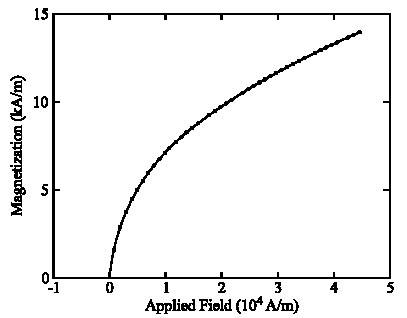
\includegraphics[width=0.65\linewidth]{images/figura1.pdf}
    \caption{Magnetización en función del campo aplicado. \\ (Observe que hay un punto después del número de figura, seguido por un espacio).}
    \label{fig:fig1}
\end{figure}

\subsection{Unidades y Notación Científica}

Para asegurar la coherencia tipográfica de las unidades en el documento, se utiliza el paquete \texttt{siunitx} (cuya documentación está disponible en \url{https://ctan.org/pkg/siunitx}). Esto evita espaciados incorrectos o saltos de línea huérfanos entre un número y su unidad:
\begin{description}
  \item[Unidades aisladas:] Se definen mediante el comando \texttt{\textbackslash unit\{...\}}. Por ejemplo, la denominación “Magnetización (\unit{A/m})” o “Magnetización (\unit{A.m^{-1}})”.
  \item[Cantidades:] Para asociar un valor numérico a su unidad, se emplea el comando \texttt{\textbackslash qty\{valor\}\{unidad\}}, como por ejemplo \qty{15000}{A/m} o \qty{0,015}{A/m}.
  \item[Multiplicadores:] Se recomienda el uso de prefijos del SI (como \unit{kA/m}) o potencias mediante la sintaxis \texttt{\textbackslash qty\{e3\}\{A/m\}}. Se debe evitar el empleo de la notación informal “$\times$ 1000”.
\end{description}
El punto intermedio ($\cdot$) para productos de unidades en expresiones como \unit{A.m^{-1}} es generado de forma automática a través de la configuración global de la plantilla.

Las figuras deben realizarse, de forma preferente, con trazos negros y fondo blanco, dado que la versión impresa suele publicarse en escala de grises. Con el propósito de mejorar la legibilidad de los gráficos, se deben emplear tamaños de letra adecuados en los ejes (entre 10 y 14 puntos), tal como se ilustra en la Fig. \ref{fig:fig2}.

\begin{figure}[h!]
  \centering
  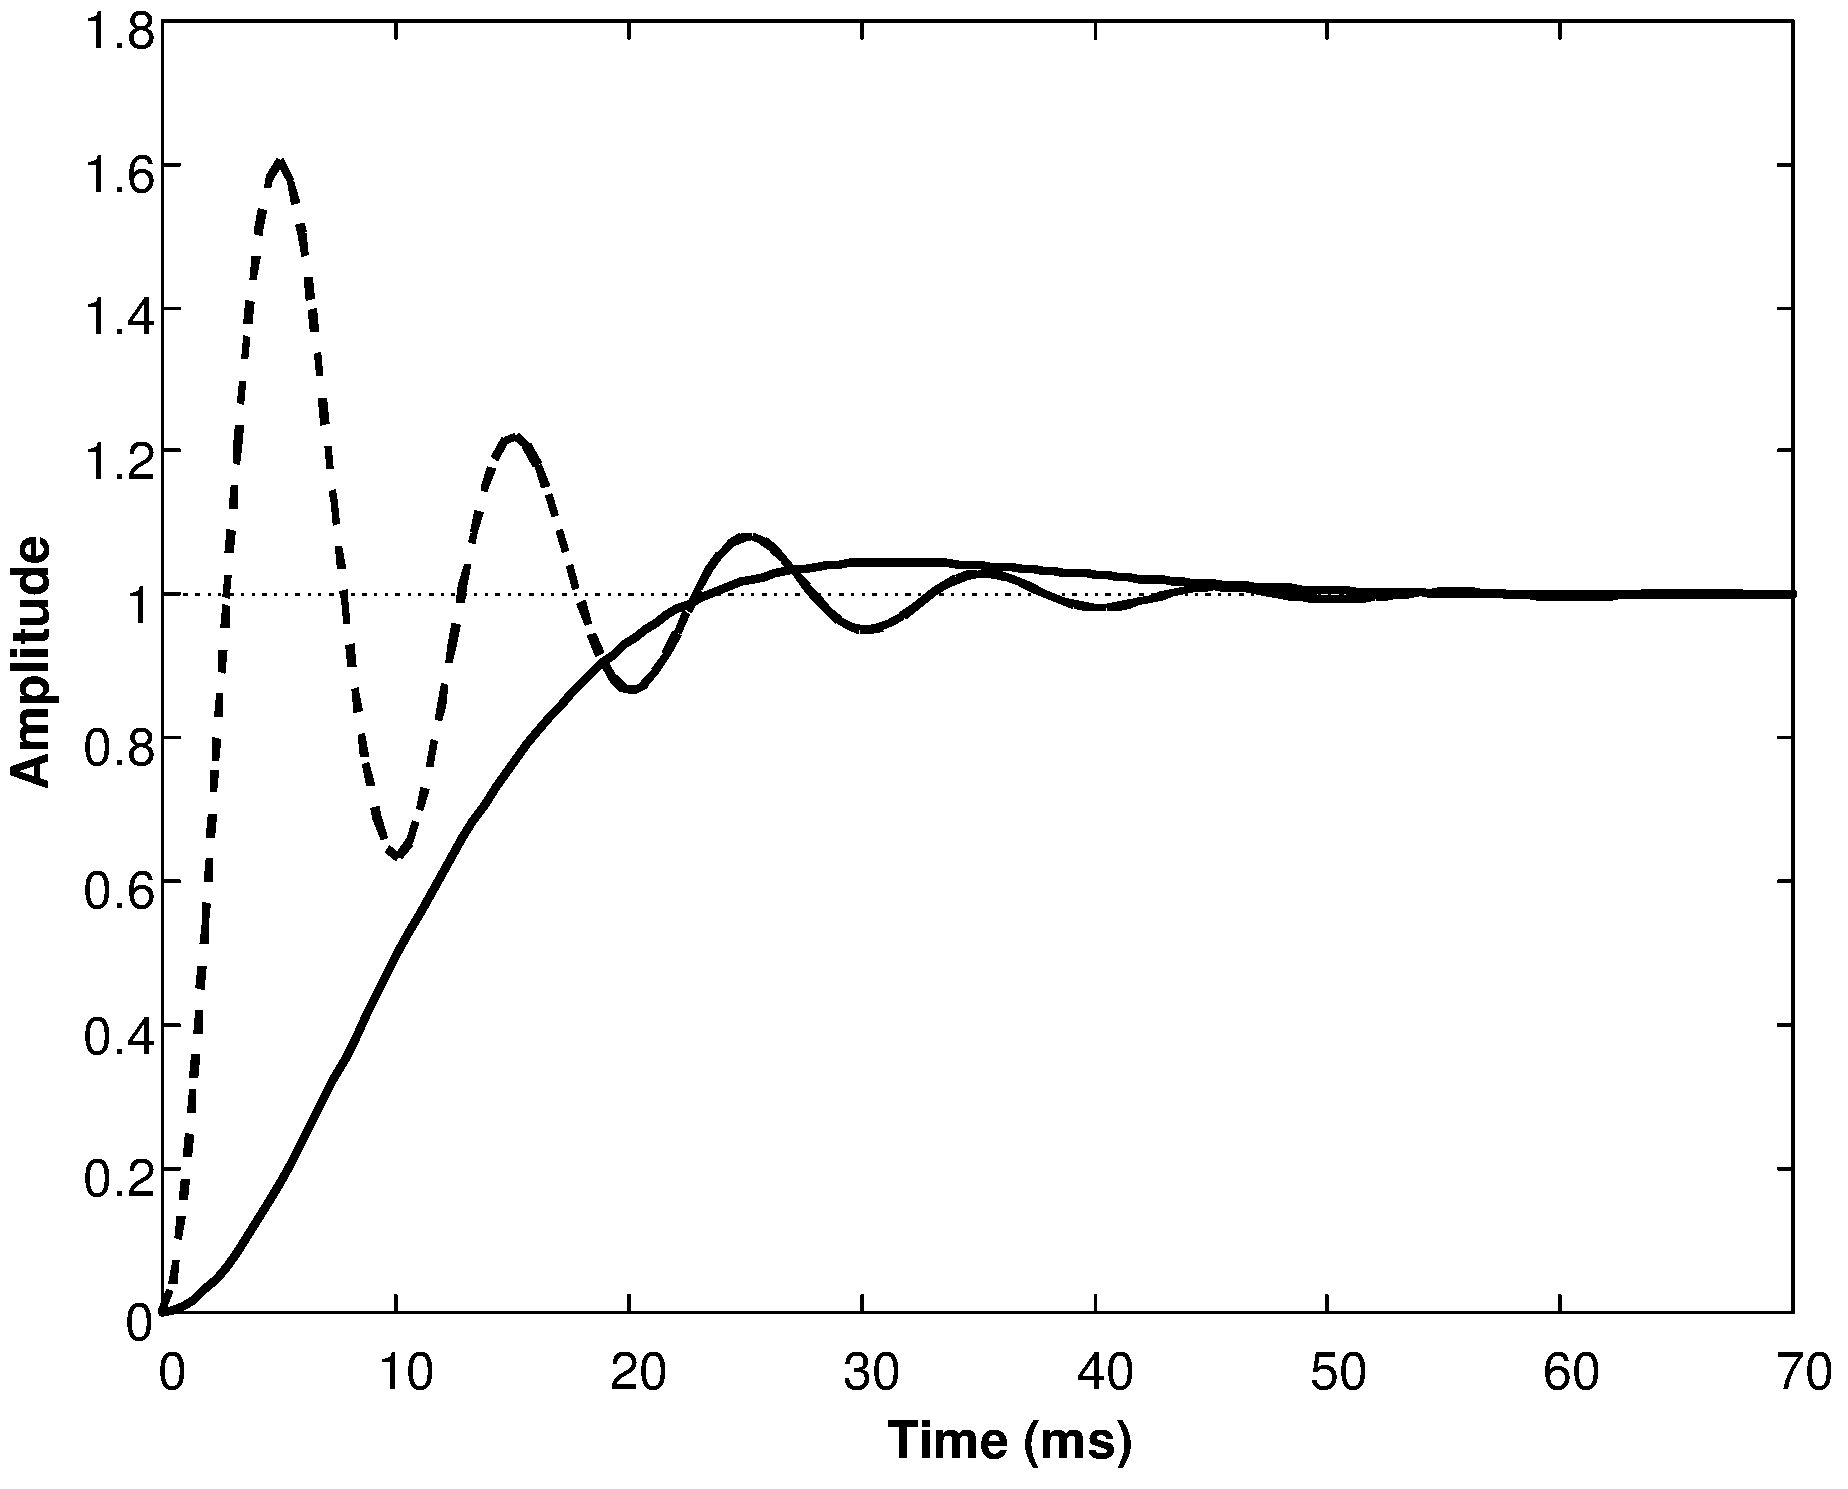
\includegraphics[width=0.65\linewidth]{images/figura2.pdf}
  \caption{Respuestas al escalón unitario del sistema de control compensado (línea continua)\\ y no compensado (línea de trazos).}
  \label{fig:fig2}
\end{figure}

\subsection{Abreviaciones y Acrónimos}

Se deben definir las abreviaturas y los acrónimos la primera vez que son introducidos en el texto, incluso si ya han sido especificados en el resumen, como por ejemplo “...Modulación de ancho de pulso (PWM)...” o “Fuentes de alimentación ininterrumpida (UPS)”. No se requiere definir siglas de uso universal como IEEE, SI, CA y CC. Las abreviaturas que incorporan puntos se escriben sin espacios intermedios (por ejemplo, “C.N.R.S.” y no “C. N. R. S.”).

Se debe evitar el uso de abreviaturas en el título, a menos que resulte estrictamente necesario.

\subsection{Ecuaciones}

En \LaTeX{}, las ecuaciones se escriben utilizando el entorno \texttt{equation}. A diferencia de otros procesadores de texto, no es necesario crear tablas para alinear las ecuaciones ni escribir los números de forma manual. El sistema centra automáticamente la ecuación y coloca el número correlativo correspondiente alineado al margen derecho, como se observa en \eqref{eq:1}.

Para estructurar ecuaciones más complejas (por ejemplo, con múltiples líneas o partes contiguas), se pueden utilizar sub-entornos como \texttt{split} (para más detalles de la escritura matemática, consulte el manual de \texttt{amsmath} en \url{https://ctan.org/pkg/amsmath}):

%%%%%%%%%%%%%%%%%%%%%%%%%%%% E C U A C I O N E S %%%%%%%%%%%%%%%%%%%%%%%%%%%%
% Las ecuaciones se escriben utilizando el entorno 'equation'.
% - \LaTeX{} numera automáticamente las ecuaciones de forma secuencial.
% - \label{eq:clave} define la clave de referencia.
% - En el texto, refiérase a ellas usando \eqref{eq:clave} para que aparezcan entre paréntesis.
% - Use 'split' para ecuaciones largas que requieran dividirse en múltiples líneas.
% - Para más información de entornos matemáticos complejos, consulte:
%   https://ctan.org/pkg/amsmath
%%%%%%%%%%%%%%%%%%%%%%%%%%%%%%%%%%%%%%%%%%%%%%%%%%%%%%%%%%%%%%%%%%%%%%
\begin{equation} \label{eq:1}
  \begin{split}
    \int^{r_2}_0 F(r, \varphi)\ dr\ d\varphi = \left[\sigma r_2 / (2\mu_0)\right]
  \end{split}
  \qquad
  \begin{split}
    \int^\infty_0 \exp(-\lambda\ |z_j-z_i|)\lambda^{-1}\ J_1(\lambda r_2)\ J_0(\lambda r_i) d\lambda.
  \end{split}
\end{equation}

Para ecuaciones simples de una sola línea, la sintaxis es directa:

\begin{equation} \label{eq:2}
  u_c(t) = K_p \left[e_v(t)+\tau_d\frac{de_v(t)}{dt}\right]
\end{equation}
donde: $u_c$ es la acción de control; $K_p$ es la ganancia proporcional; $e_v$ es la señal de error de tensión y $\tau_d$ es la constante de tiempo derivativa.

Para la escritura matemática en el manuscrito, se deben considerar las siguientes recomendaciones:
\begin{description}
  \item[Signos de puntuación:] Las ecuaciones que forman parte de una oración deben finalizar con el signo de puntuación correspondiente (coma o punto), tal como se muestra en \eqref{eq:1}.
  \item[Variables y Constantes:] Por defecto, el modo matemático presenta las variables en cursiva, lo cual es adecuado para parámetros físicos (por ejemplo, $t$ o $T$). Las constantes matemáticas y unidades físicas se deben escribir en letra redonda (por ejemplo, la unidad de inducción magnética se escribe $\mathrm{T}$ o utilizando el comando \texttt{\textbackslash unit\{\dots\}}).
  \item[Vectores y Matrices:] Se recomienda representarlos con tipografía en negrita empleando comandos como \texttt{\textbackslash mathbf\{\dots\}}.
  \item[Referencias a ecuaciones:] Se debe emplear siempre el comando \texttt{\textbackslash eqref\{clave\}} en lugar de transcribir la numeración manualmente. Esto genera automáticamente los paréntesis y el enlace de hipertexto (por ejemplo, “el resultado de \eqref{eq:1}”). Asimismo, se aconseja evitar términos como “Ec. \eqref{eq:1}” o “ecuación \eqref{eq:1}”, a menos que se sitúen al inicio de una oración (por ejemplo, “La ecuación \eqref{eq:1} representa\dots”).
\end{description}

\subsection{Otras Recomendaciones}

\begin{description}
  \item[Espaciado:] Se debe emplear un único espacio después de los signos de puntuación. El motor de compilación de \LaTeX{} ajusta el espaciado entre palabras de manera óptima.
  \item[Redacción técnica:] Se debe evitar el uso de gerundios o participios de forma incorrecta para la descripción de metodologías (por ejemplo, “Usando \eqref{eq:1}, se calculó el potencial”, donde no se identifica el sujeto de la acción). En su lugar, se recomiendan estructuras como: “El potencial se calculó mediante \eqref{eq:1}” o “A través de \eqref{eq:1} se obtuvo el potencial”.
  \item[Justificación automática:] En \LaTeX{} la justificación tipográfica, la separación silábica y la distribución del texto son procesadas automáticamente por el motor TeX. Se debe evitar la inserción forzada de saltos de línea con \texttt{\textbackslash\textbackslash} dentro del párrafo, así como la adición de guiones o espacios manuales con fines de alineación.
\end{description}

\section*{Agradecimientos} % Opcional

Este trabajo ha sido llevado a cabo gracias al apoyo de la Agencia Nacional de Promoción de la Investigación, el Desarrollo Tecnológico y la Innovación (ANPCyT). 

Los autores agradecen a Samuel Jackson por la colaboración prestada en la preparación de este artículo.

\appendix
\renewcommand\thesection{Apéndice \Alph{section}} % Incluir 'Apéndice' en la etiqueta

\section{Título del Primer Apéndice}
En esta sección usted puede escribir el texto y ecuaciones relacionadas al primer apéndice.

\section{Título del Segundo Apéndice}
En esta sección usted puede escribir el texto y ecuaciones relacionadas al segundo apéndice.

%%%%%%%%%%%%%%%%%%%%%%%%%%%% R E F E R E N C I A S %%%%%%%%%%%%%%%%%%%%%%%%%%%%%

% Las referencias viven en el archivo `references.bib`, puede incorporar
% diferentes tipos de recursos siguiendo el formato biblatex, similar a JSON,
% en ese archivo y luego hacer mención a ellos en el texto del artículo
% utilizando el siguiente comando: \cite{id-recurso}

% Las citas se enumerarán de forma automática según el orden de aparición
% en el artículo y se presentarán en esta sección utilizando el formato IEEE
% incluyendo la información presente en el archivo `references.bib` para
% el recurso citado.

% Para ver más acerca de qué tipos de recursos son soportados y qué
% parámetros están disponibles para ellos consulte la documentación:
% http://mirrors.ctan.org/macros/latex/contrib/biblatex/doc/biblatex.pdf

% Referencias no citadas no deben ser incluidas en esta sección, para ello
% elimine o comente la siguiente línea al incorporar sus propias referencias
\nocite{*} % <-- Sólo a modo de ejemplo, eliminar o comentar

\printbibliography

\end{document} % Máx. 15 páginas
